% Der Zertifizierung nach dem deutschen Eichrecht entsprechend, muss jede Ladesäule auf Eichrechtskonformität (ERK) überprüft werden.
% Dieser Prozess wird immer wieder auf die gleiche Art und Weise im gleichen Umfang durchgeführt. 
% Er beinhaltet somit ein entsprechendes Automatisierungspotential.

Der OCPP Server als Bibliothek soll in eine andere Software integriert werden, 
um mithilfe der ausgetauschten Nachrichten das Verhalten der Ladesäule (im allgemeinen Sinne) auswerten zu können.
Es werden nicht alle Funktionalitäten des Servers benötigt. 
Die Software beinhaltet neben der OCPP Schnittstelle (mittels Bibliothek) auch weitere Schnittstellen.

% Dafür muss für jede Ladesäule ein Ladevorgang gestartet werden (Transaction), währenddessen Strom fließt und gemessen wird.   
% Um die Datenintegrität der Messwerte und deren Transport sicherzustellen wird der OCPP Server verwendet. 
% Mit dessen Hilfe kann nachgewiesen werden, 
% dass die Daten nirgendwo in der Software geändert und ebenso unverändert an den Server übertragen und dort abgerechnet wurden. 
% Nach Beenden der Transaction werden mittels einer Drittsoftware die gemessenen Daten mit den Transactiondaten verglichen.

% Die Anforderungen an das Automatisierungstool sind:
% \begin{itemize}
%     \item Leichte Bedienbarkeit der Software
%     \item Leicht Integrierbar in das andere Automatisierungstool
% \end{itemize}

Die Anforderungen an die Bibliothek sind:
\begin{itemize}
    \item OCPP Server soll parametrierbar sein
    \item OCPP Nachrichten sollen im Cache gespeichert werden können
    \item Leichte Integrierbarkeit in die andere Software
\end{itemize}

Die nachfolgende Abbildung \ref{fig:summaryDiagrammLibrary} ist ein Übersichtdiagramm der Software.
\begin{figure}[H]
    \centering
    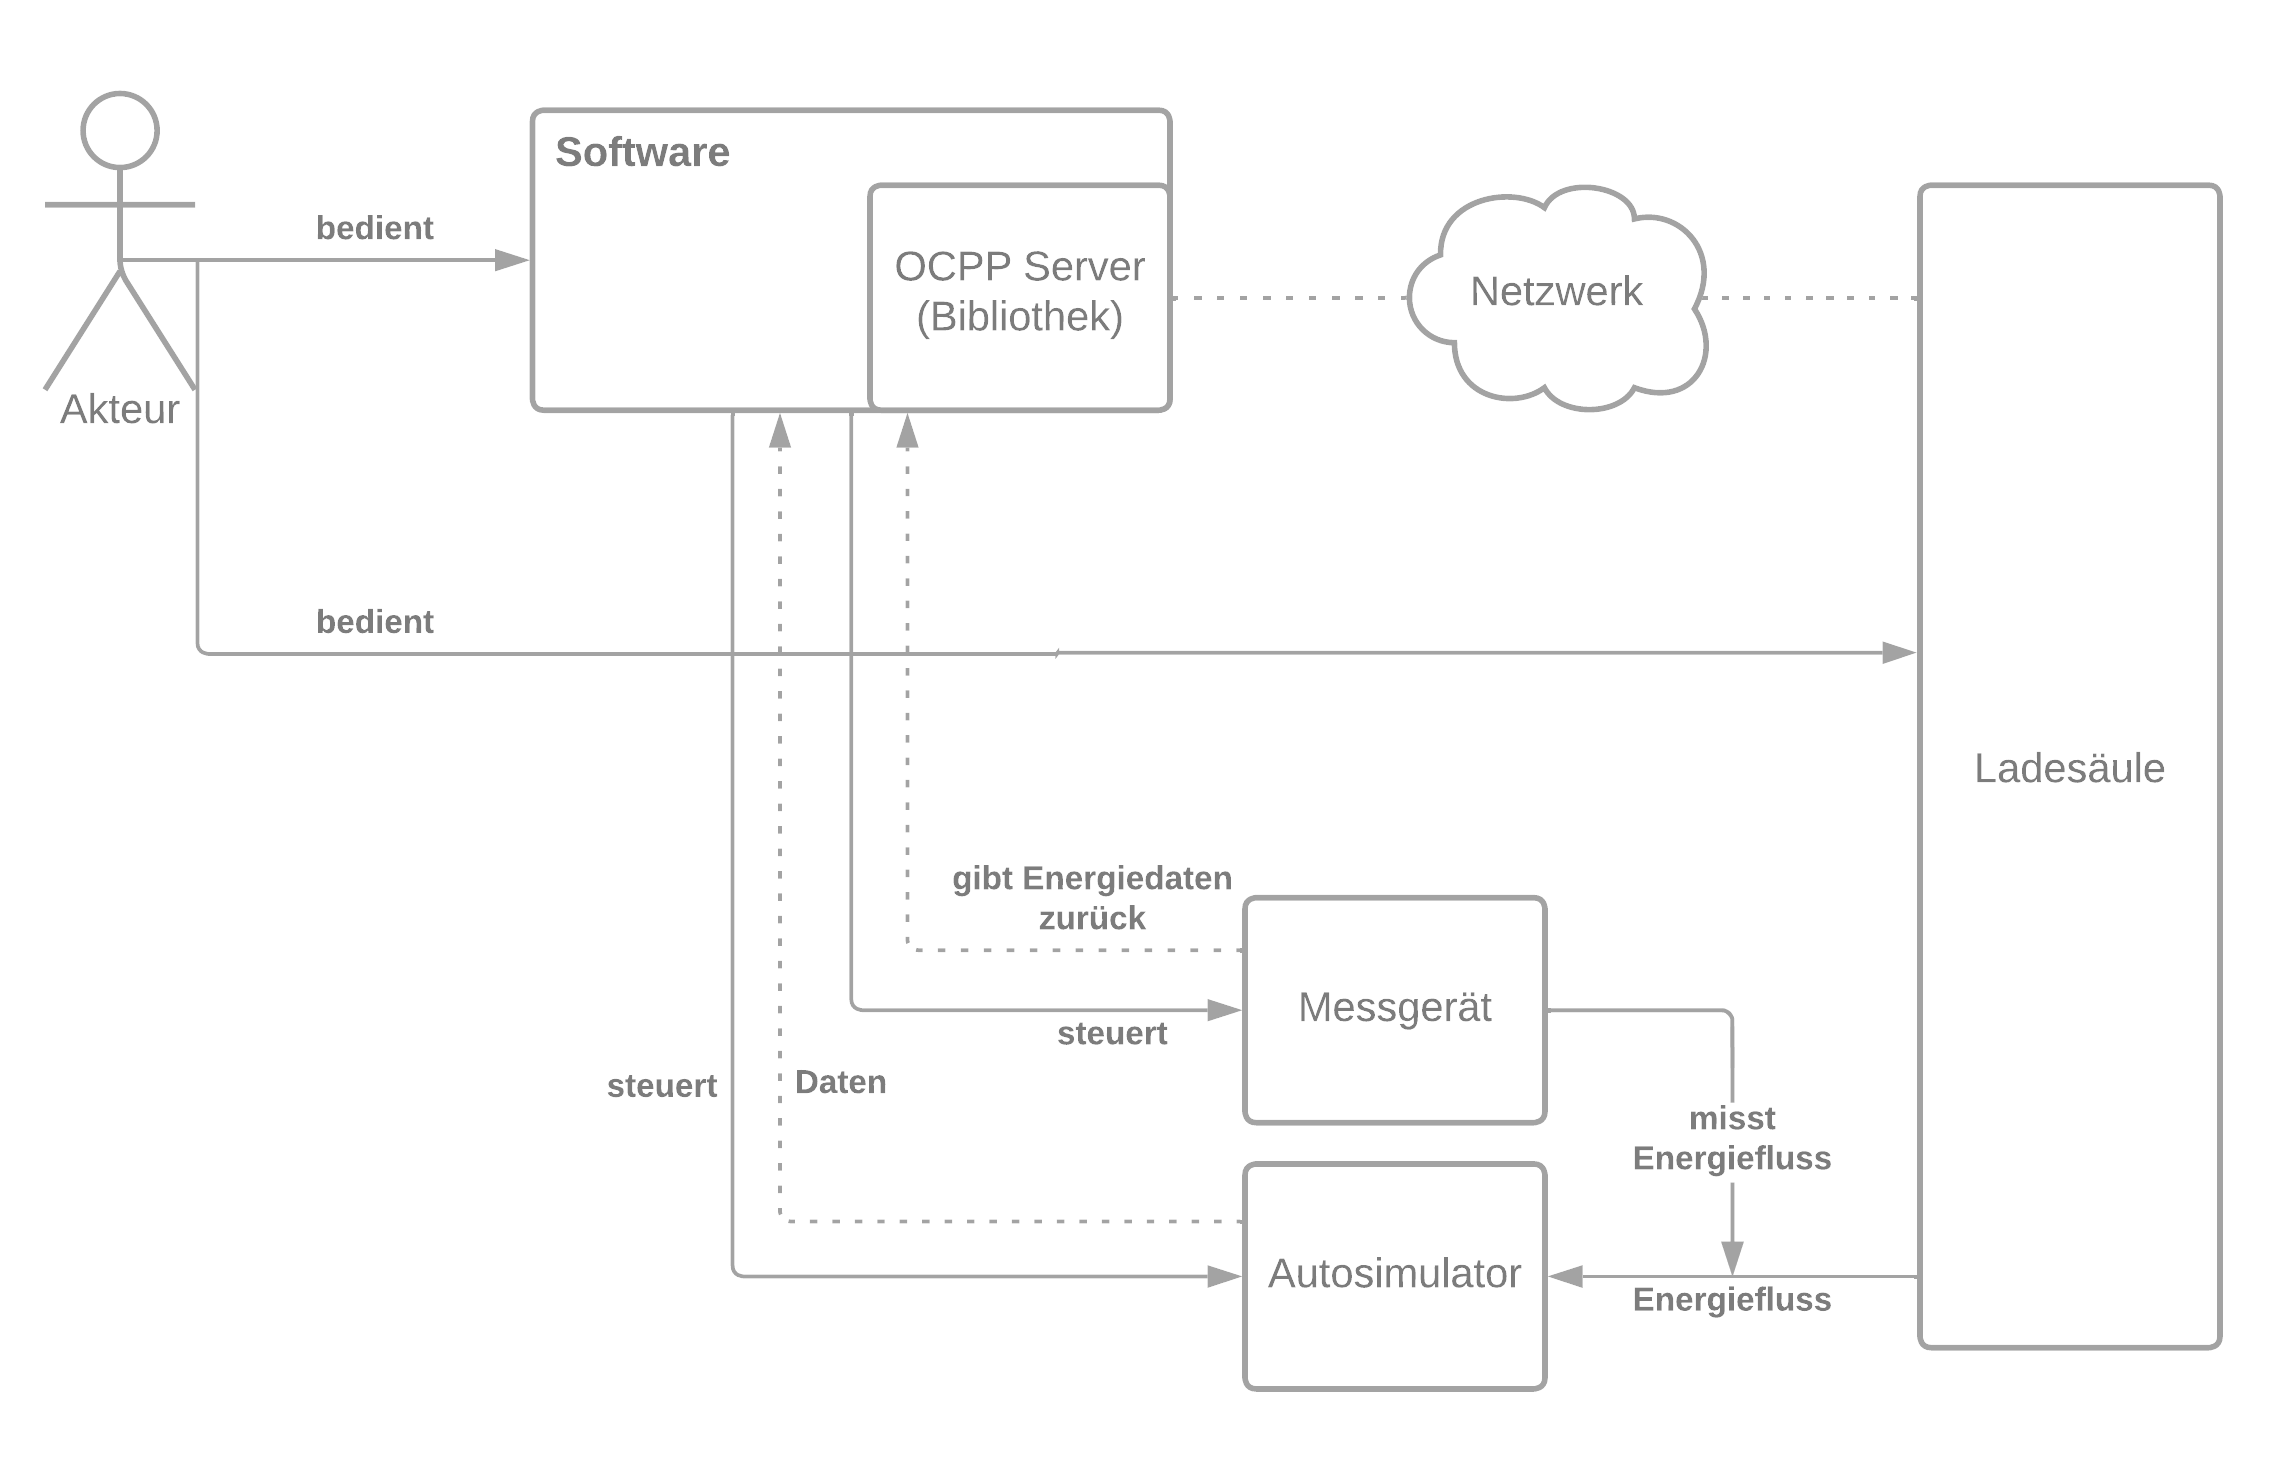
\includegraphics[width=1\textwidth]{./images/ERK.png}
    \caption[Übersichtdiagramm der Software]{Übersichtdiagramm der Software}
    \label{fig:summaryDiagrammLibrary}
\end{figure}